%!TEX root = ../../dissertation.tex
%%%%%%%%%%%%%%%%%%%%%%%%%%%%%%%%%%%%%%%%%%%%%%%%%%%%%%%%%%%%%%%%%%%%%%%%%%%%%%%%
\section{Measurements}
\label{c3:measurements}

With these playback models at hand, this section demonstrates how to conduct actual evaluations of reliable streaming protocols with it.

As discussed, there are numerous incarnations of reliable streaming protocols in use. Almost all of them follow the same basic approach but with slight variations in execution and choice of playback strategies and corresponding parameters. But it is exactly these choices that can have a large impact on the streaming process and resulting quality. 

The problem lies in comparing these protocols to each other. Each of them is usually tied to a specific -- and most often proprietary closed source -- streaming player. Setting up all these players in one testbed is a huge effort and requires very specific software environments to be used on the client machines. Moreover, these players are built with user interaction and not automation and directly measuring the outcome in mind. This can still be achieved through extensive workarounds, but must be tailored to every player application. The presented approach avoids this hassle and provides a concise way to test any conceivable playback strategy in one single test setup.



%%
\subsection{Progressive Streaming Measurement Framework}

To enable quick evaluations for progressive streaming the framework follows a two phase approach, separating the active online recording phase from the passive playback emulation. Recording data is very time intensive and cannot be sped up when conducting investigation of a real world process, and not relying on simulated data. It still replicates the steps a user would perform to consume a media stream on a playback device. Through appropriate configuration different scenarios can be modeled, e.g. network conditions, behavior and specifics of the user device.
 
\begin{figure}[htb]
    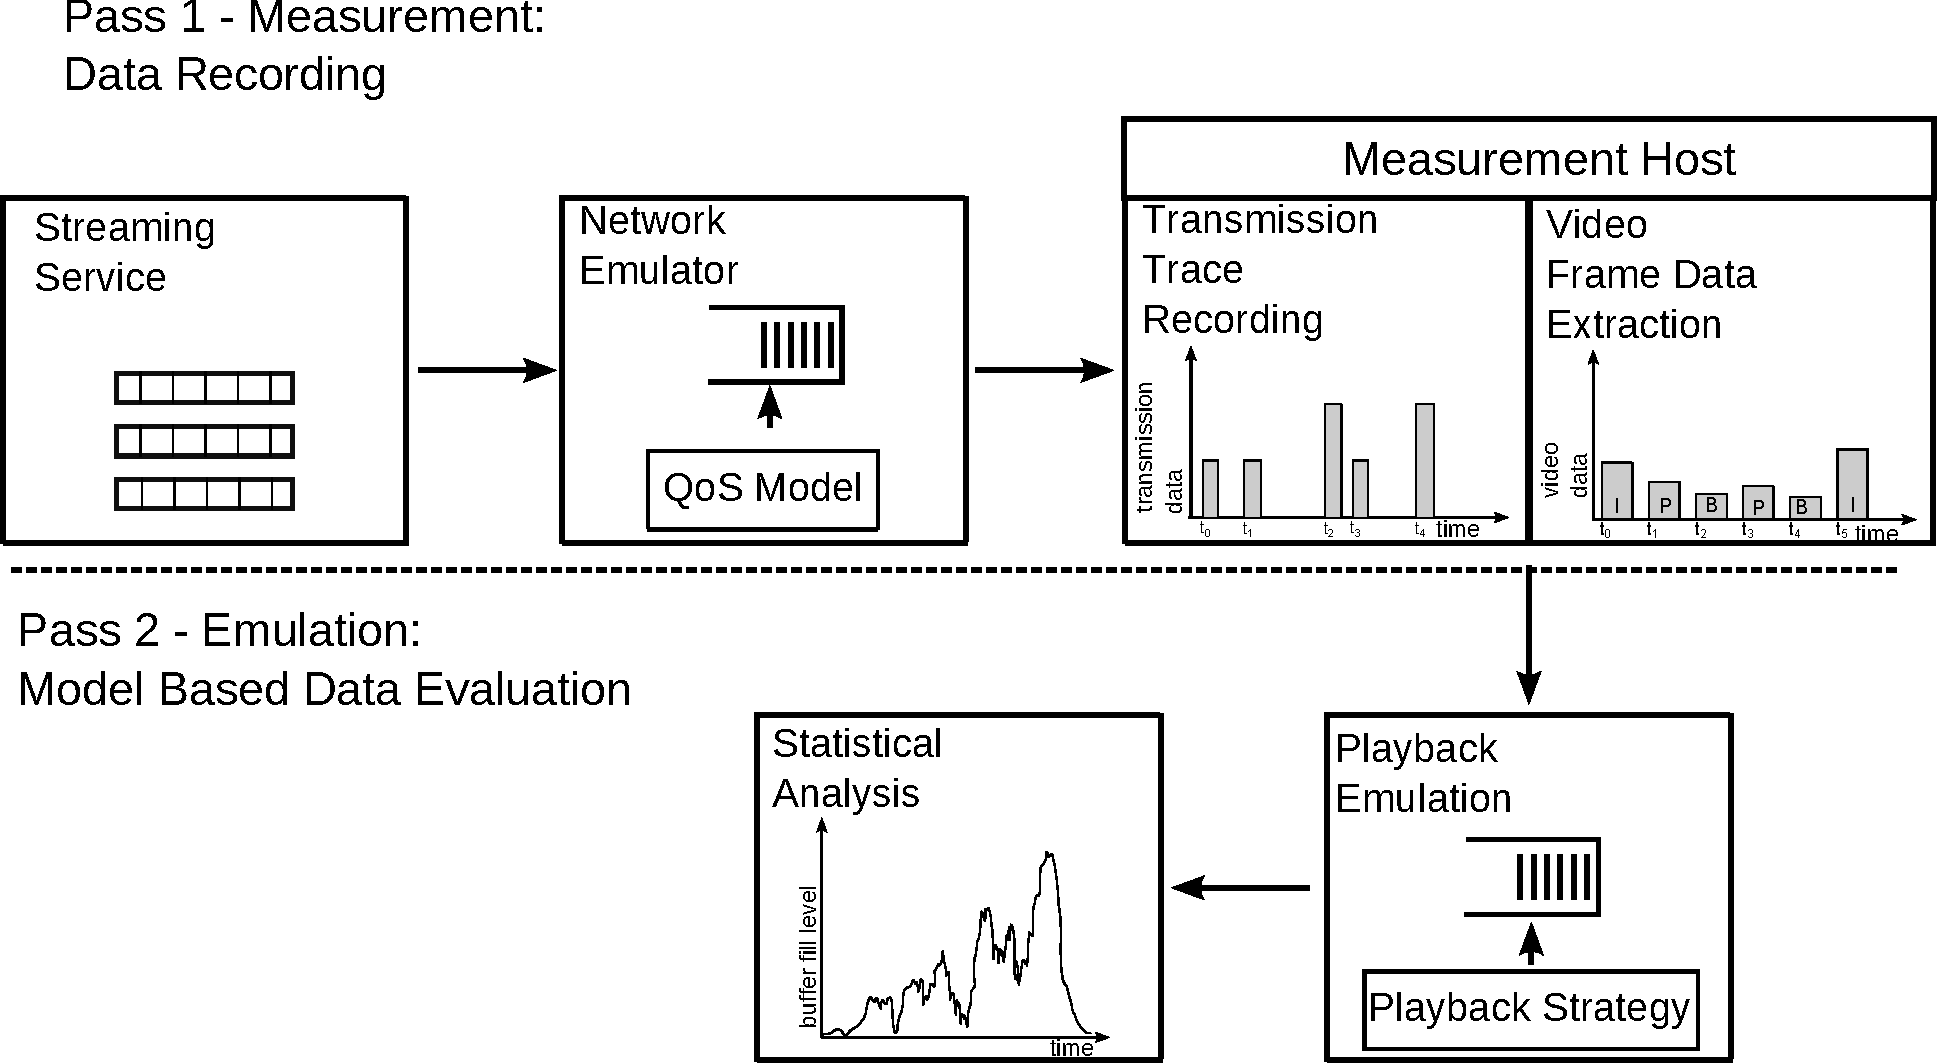
\includegraphics[width=\textwidth]{images/measurement-model.pdf}
    \caption{Measurement framework for progressive streaming playback strategies overview.}
    \label{c3:fig:framework}
\end{figure}

Figure \ref{c3:fig:framework} depicts the framework for a streaming evaluation testbed. In phase one the stream's transmission is conducted and recorded on a per-packet level. Stream data is transmitted to the client from a server which can be any actual streaming service on the Internet or a local server under the testbed's control, eliminating undesired side effects caused by the Internet connection. 

The traffic is directed through a network emulation node capable of altering the network QoS parameters, i.e. latency, jitter, and packet loss. The parameters could also be set according to stochastic models derived from actual network traces. Instead of network emulation, any preexisting architecture can also be placed here to achieve more accurate results for the intended target. This is especially helpful for complex infrastructures hard to model or with no good and concise models available yet, for example mobile and mobile core networks.

The measurement host downloads and records the video stream as a network trace. For progressive \gls{HTTP} streaming, a single request on the video file is issued and the \gls{TCP} connection maintained until the file has fully arrived.
This process is recorded in traces as basis for the second phase. A trace should consists of the size and timestamp of every incoming packet. More detailed traces can be used to scrutinize other layers of the connection, e.g. the dynamics of TCP receive window size. Additionally the received file is decoded yielding a trace of the video frame sizes and playout timestamps.

%% <-- WIP


In the second pass, these two traces are then used to feed the playback models described before. The playback emulation process combines the transmission and video frame traces to calculate the playback buffer fill level for every point in time during the playback. It then generates statistics about user-perceivable artifacts such as playback stalls that would occur during the playback. These statistics can then be compared to the results of other models and network QoS.

% For simple HTTP streaming, there is no feedback from the client to the server that would result in adaptions of the stream (``rate control''). Therefore, recording the packet trace and simulating playback are decoupled, as the latter cannot influence the former. As such, the testbed can test and compare several playback models on the same recorded network trace. This enables fast and efficient comparison of non-feedback protocols subject to the same network conditions.



Which metric to compare strategies and to record during experiments? Time, number and duration of stalls, buffer fill level.

Which experiment parameters to change and test for? Network \gls{QoS}, meaning bandwidth, latency distribution, loss; strategie parameters on the other hand --> could empirically test every parameter combination, improve it and feed it back into the testing framework; emulate specific network conditions, e.g. mobile 3g/lte network + signaling/control plane, middlebox influences
 Through configuration, one may evaluate the influence of network parameters, states, and topologies on the multimedia stream, e.g. parallel bearers with different quality settings, cross traffic, or stream-support middleboxes.


drawback: first need to find out the exact playback strategy from the player under investigation (if player is tested and not mechanism in general)
model, compare performance based on behavioral, structural commonalities

for offline (or no feedback strategies) two pass process, online trace recording and offline emulation/simulation phase
allows for very fast evaluation of a strategy subset

record a large number of traces to compare adaptability to many scenarios or just to a specific one

playback emulation: just caluclate buffer level: speed up versus actual playback but the same outcome



%% <-- %% end WIP



%%
\subsection{Online Framework Extension}

define feedback: any strategy, that alters transmission (i.e. requesting segments/ranges; when to request, parallel request, quality to request) based on current conditions

modifications for adaptive/segmnet-based/feedback streaming

can use server under own control, to influence server side pacing

no trace phase anymore, (emulated) transmission phase now part of old phase 2


\begin{figure}[htb]
    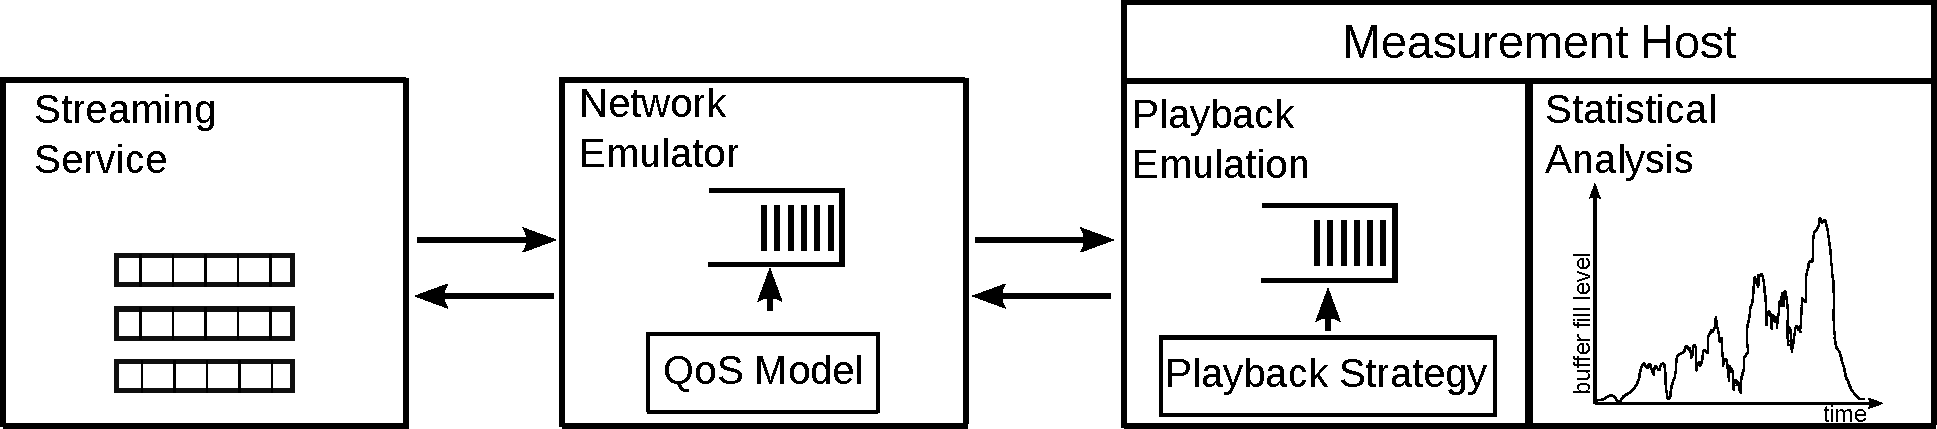
\includegraphics[width=\textwidth]{images/feedback-measurement-model.pdf}
    \caption{Measurement framework for adaptive streaming playback strategies overview.}
    \label{c3:fig:framework-feedback}
\end{figure}


Figure~\ref{c3:fig:framework-feedback}


\subsection{Transition to Full Simulation}

\subsection{Technical Implementation}

3 linux nodes, python emulation, netem module, curl, ffmpeg, mplayer, R
event based emulation?

describe network emulation (and specifically netem)



%%
\subsection{Measurement Series and Evaluations with the Framework}
%[visualization and results (does yt still work well with high delay/loss?)]
%[performance evaluation (BWs, played vs received data)]
%Also observed and analyzed. The deduce that the initial buffering time and the later block sending rate are directly correlated. 64kb blocks, probably due to GFS, problems with this method, ...
%These Quality-of-Service parameters loss and delay do not have any direct influence on the downloading process but instead have negative impacts on the throughput of the underlying TCP due to its congestion control feature and, in the end, serve as another source of delay and jitter.

For the YouTube streaming measurements we implemented an automated video downloading and playback simulation software to feed information into the model and evaluate the total stalling time. For this the simple stalling model is used because this results in the shortest possible playback duration in every scenario. Furthermore, we used a network emulation testbed to subject the video streaming to increased loss and latency while fixing the maximum network bandwidth and observe the influence on the QoE.

First use case to show how our system works: Progressive HTTP streaming. Will show adaptability to adaptive streaming and different protocols. For this comparison we used a video of about 90 seconds length and network conditions that could not fulfill the video bitrate in time and hereby forced stalling to occur.

We performed two measurement series, one with increased packet loss, the other one adding latency to the path. For each value of loss and latency a mean total stalling time was calculated out of five separate experiments to eliminate temporal and network load influences. Additionally, standard deviations are shown in the resulting graphs. We clearly notice very large deviations in some experiments. Some of these can be explained by connection timeouts and later resumption of the streaming. Furthermore, an exponential regression line shows the trend of the total stalling times in the experiments.

\begin{figure}[htbp]
% yt-delay-allBW.ods, graphik aus LibreOffice Calc, OLE in LibreOffice Draw, font sizes min 11pt, Page Margins passen (18,2 x 10,3), als PDF exportiert.
% new method: extra libreoffice calc page, scaled to fit on one page, pdf export, cut with acrobat
    \centering
    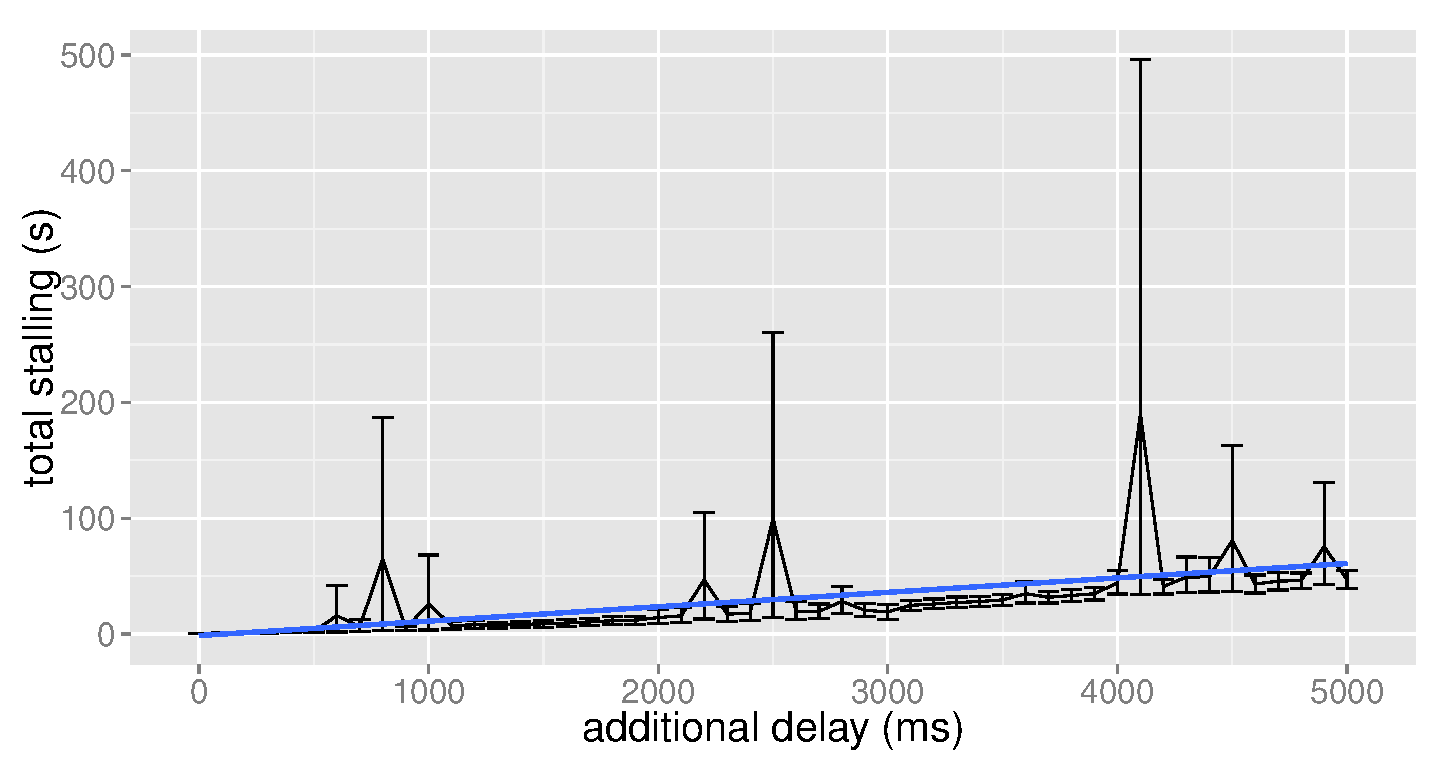
\includegraphics[width=\textwidth]{images/R-delayseries.pdf}
    \caption{Total buffering time and linear smooth for degraded network parameter scenarios. Latency Graph.}
    \label{c3:fig:delayseries}
\end{figure}

\begin{figure}[htbp]
    \centering
    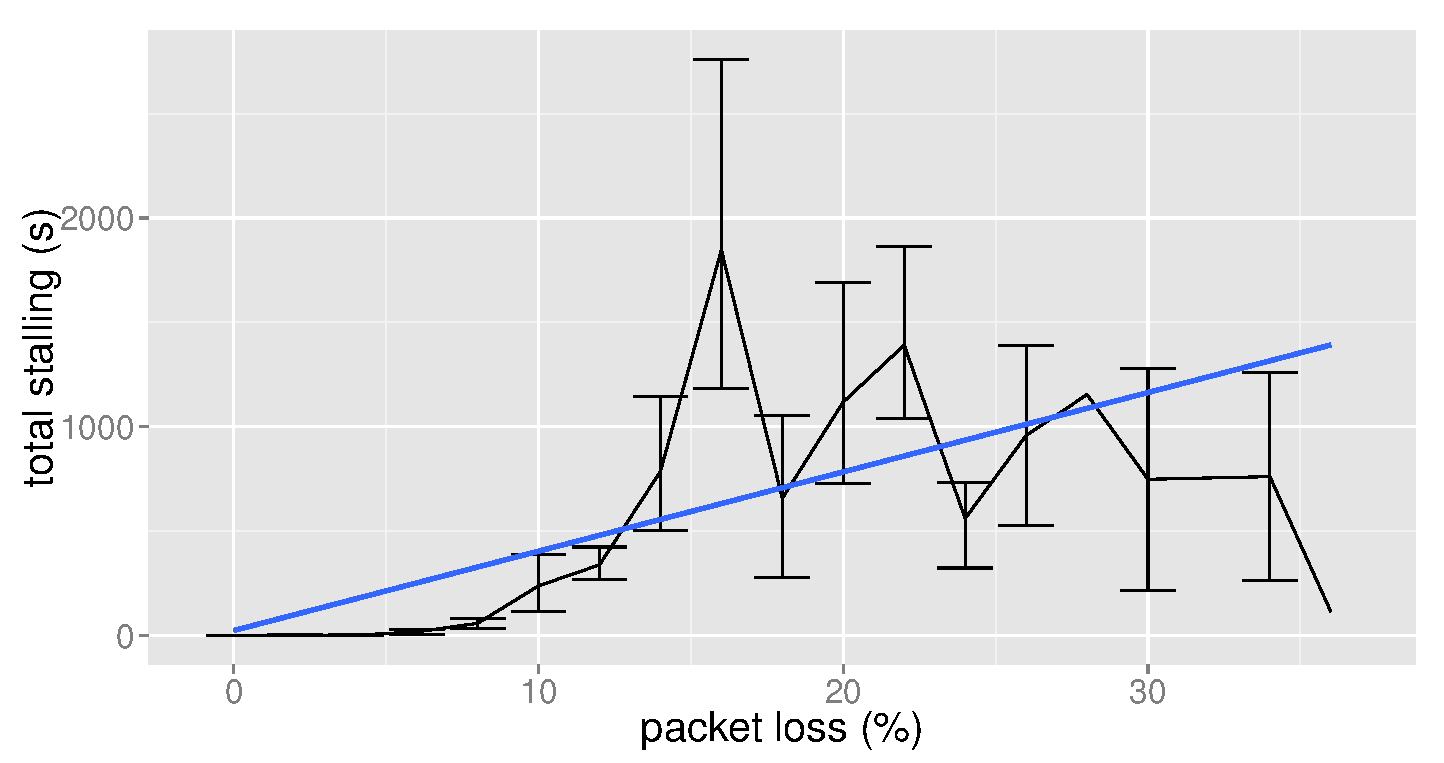
\includegraphics[width=\textwidth]{images/R-lossseries.pdf}
    \caption{Total buffering time and linear model for degraded network parameter scenarios. Loss Graph.}
    \label{c3:fig:lossseries}
\end{figure}

Figure \ref{c3:fig:delayseries} displays the results of of the latency measurement series with up to five seconds of additional delay. In the worst case the stalling time increases to about 50 seconds. In mobile scenarios latencies of up to 2 seconds can be expected, which would, according to our measurements, result in a maximum mean stalling time of 15 seconds for a 90 second video, which could very well be bearable for YouTube users.

There are several factors that could contribute to the increase in stalling time in the latency experiments. 
TCP, in its simplest form, increases the congestion window based on the Round Trip Time (RTT), making it highly dependent on this connection parameter. Newer congestion avoidance algorithms, e.g. the CUBIC algorithm used in Linux \cite{ha2008cubic}, however reduce this dependence on the RTT.
Another influencing factor might be YouTube's block sending mechanism, which, according to \cite{alcock2011afcyt}, may negatively interact with congestion control algorithms. The impact of packet loss on stalling is much higher than that of latency in our measurements. Yet, due to TCP's reliable transmissions, loss only causes increased packet retransmissions, and, thus, acts as a source of burst delay which negatively impacts the overall throughput.

Figure \ref{c3:fig:lossseries} shows the series of loss experiments. While the 6\% packet loss and below has an almost negligible influence on the stalling time anything above this value will probably not achieve good user experience at all. Interesting to note is the rather sudden increase in stalling time when there is more than 6\% loss added. This could again hints to the transport protocol's reliable transport feature, which catches all the occurring losses, through timeouts or gaps in the sequence numbers. However, the detection and retransmission takes some time, which is reflected in the increased stalling time.



The results presented here show some of the capabilities in comparing play network conditions based on playback models. We compare how the four playback models introduced previously fare against each other in a measurement series featuring  emulated transmission latency and packet loss . At the same time, we acknowledge that other specific questions are not touched in this first set of experiments, e.g. the inclusion of a mobile network or handset, or RTP-based streams.

The video used in our measurements was streamed from the YouTube web site. This provides a realistic base for all the experiments. Note that YouTube also employs its own form of application layer flow control in addition to TCP's \cite{alcock2011afcyt}. % The influence of the access bandwidth can mostly be neglected with this mechanism as long as the limit is well above the video bitrate, which was the case here.
Details on the streamed video are available in Table \ref{c3:tbl:videoparams}.

\begin{table}[htbp]
    \centering
    \caption{Test Video Parameters}
    \label{c3:tbl:videoparams}
    \begin{tabu}{|l|X[r]|}
        \hline
        Parameter & Value \\ \hline
        Video Duration  & 01:32.536 minutes \\
        Size & 9.61 MiB \\
        Framerate & 23.976/s \\
        Average Video Bitrate & 871 Kbps \\
        Codec & AVC+AAC \\ \hline
    \end{tabu}
\end{table}

For the loss experiment series, the network emulator was configured to drop a certain percentage of packets based on a normal distribution on both the uplink and the downlink direction. There was no loss correlation involved, the existence of which one would expect, e.g., in wireless networks. One streaming run for every two percentage points of additional loss up to 14\% was conducted.
In the latency series, the emulator delayed the delivery of every packet for a set constant amount of time. Half of the total amount is added to the uplink the other half to the downlink. One experiment was conducted for every 100ms of additional delay, up to a total of 5000ms.

After the traces were recorded, every playback model was applied to all runs. For every model, two data points were computed. First, the total stalling time was calculated. This is the time the player keeps buffering and not playing the video, including the initial start delay. To attain results comparable to the other measurements, the stalling time is calculated relative to the total video length instead of an absolute value. The second resulting value is the number of times the video stops playing including the initial delay, i.e. the stalling frequency. Both of them are an indicator how well the playback mechanism can cope with the currently emulated network setup. They could for example be used to either check if a modification to a network has a noticeable impact on streaming experience, or to find an optimized player behavior for a given network.

All models will generally work very similar in good network conditions. If sufficient bandwidth is available, they will play videos with almost no delay and  intermediate buffering. If, however, the achievable TCP goodput is close to the average video bitrate, the buffer may be strained by short deviations from the average rates. %TCP goodput can also be severely limited by high latency and loss. Many TCP congestion control algorithms depend on the round trip time. If the RTT is high, the congestion window will increase much slower.

High latency can also trigger TCP timeouts and retransmissions, and in turn decrease the congestion window, further impacting the goodput. The latency measurements are depicted in Figures \ref{c3:fig:eval-latency-stallingtime} and \ref{c3:fig:eval-latency-numstalls}. The stalling time increases with the additional latency. The Initial Start Delay model provides the best possible result in terms of pure stalling time. On the other hand, Figure \ref{c3:fig:eval-latency-numstalls} shows the Stalling model provides always the worst result for the number of stalls. Any other model will lie beyond that line. The Flash and HTML5 models both run in just a few buffering events which however tend to increase in length with rising latency. Attributed to the simple and optimistic assumption of the Flash model, stalling time is usually lower than with HTML5, at the cost of slightly more buffering events.
 

\begin{figure}[htb]
    \centering
    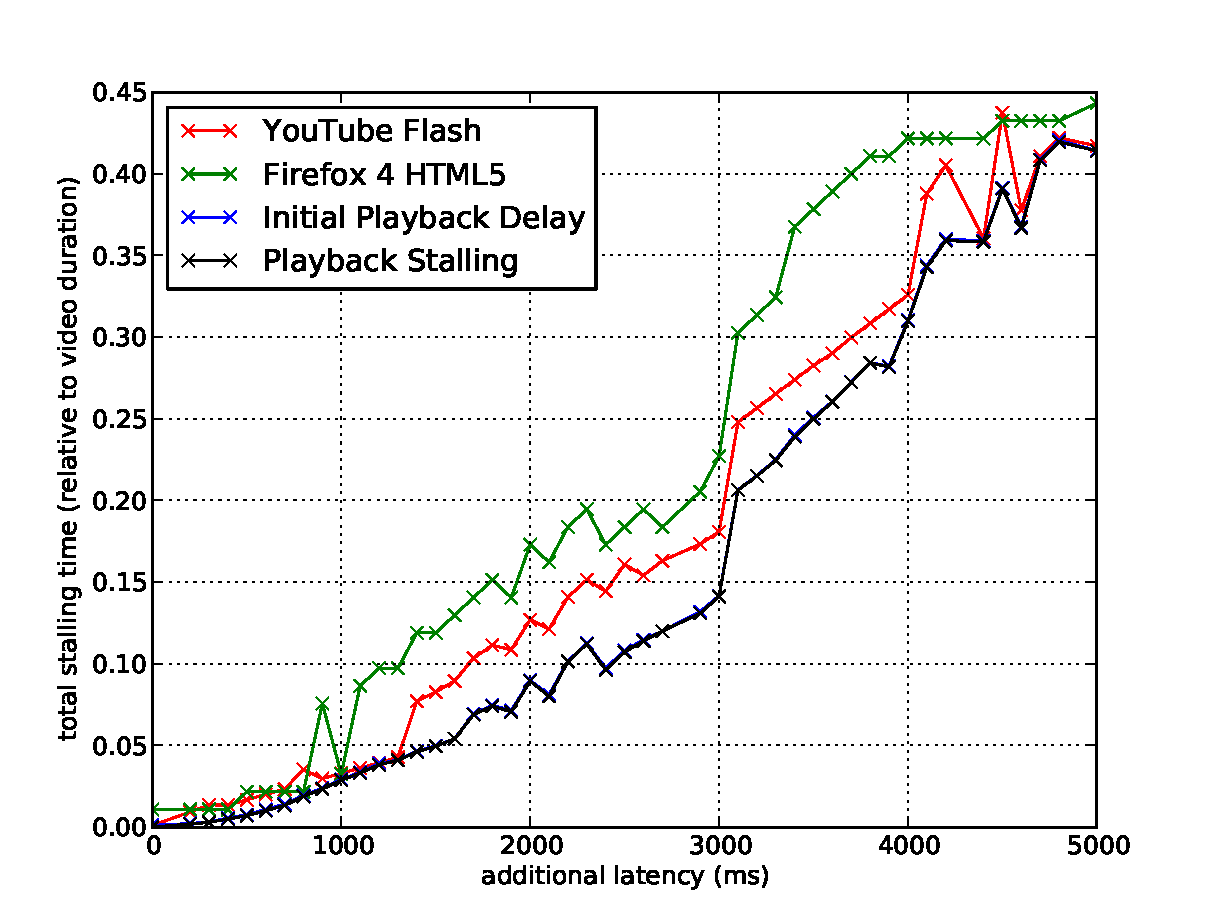
\includegraphics[width=\textwidth]{images/eval-latency-stallingtime.pdf}
    \caption{Total stalling time.}
    \label{c3:fig:eval-latency-stallingtime}
\end{figure}

\begin{figure}[htb]
    \centering
    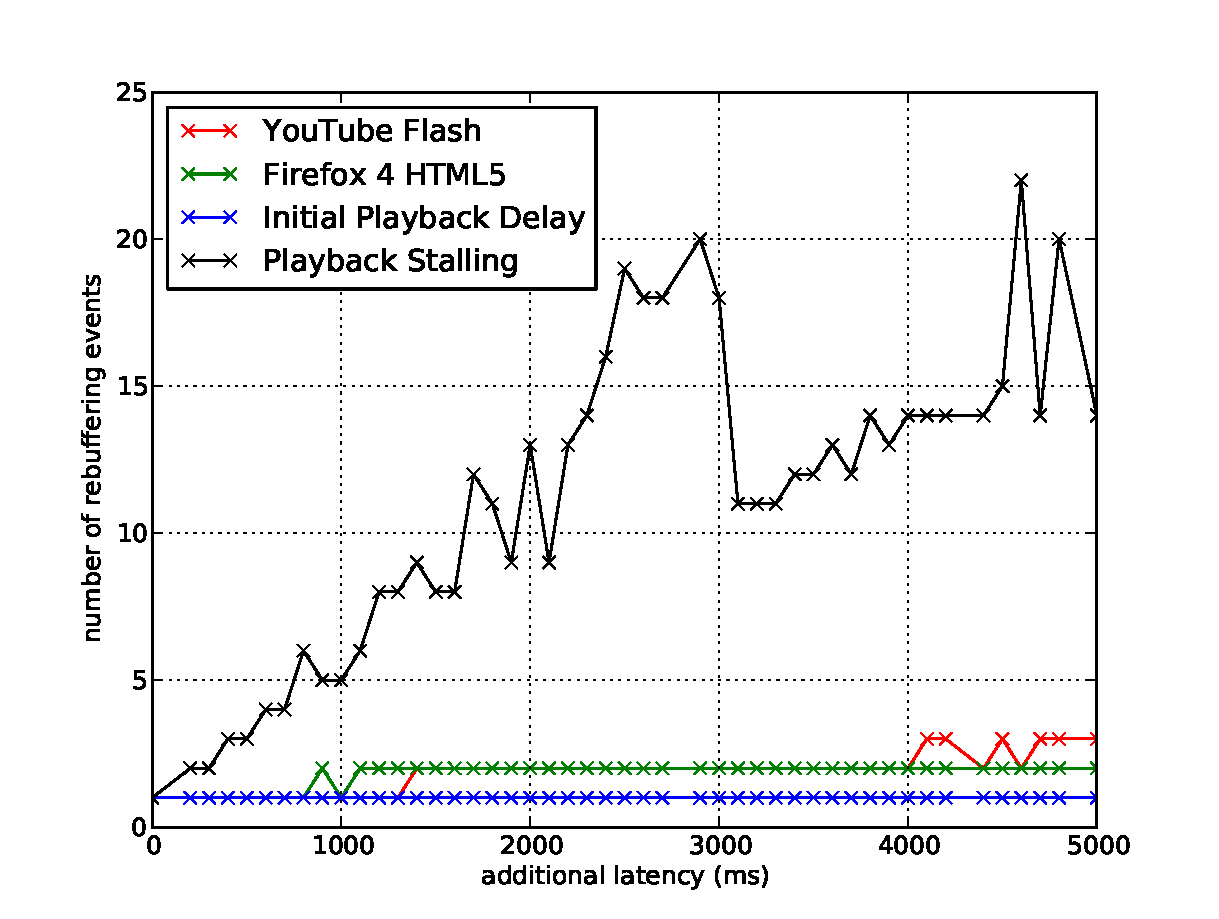
\includegraphics[width=\textwidth]{images/eval-latency-frequency.pdf}
    \caption{Playback model observations on additional latency. Number of stalls.}
    \label{c3:fig:eval-latency-numstalls}
\end{figure}


TCP goodput is even more severely affected by packet loss. A lost packet results in a duplicate acknowledgement, retransmissions, and a decrease of the congestion window. The problem gets worse if also the ACKs are lost and the connection stalls on missing old segments without which the playback cannot proceed. Figure xyz shows some exemplary measurements for a loss scenario. While additional packet losses of up to four percent seem to have no noticeable impact on streaming quality, the total stalling time suffers a large increase for any model as seen in Fig. \ref{c3:fig:eval-loss-stallingtime} rendering any streaming attempts practically unusable. Figure \ref{c3:fig:eval-loss-numstalls} shows the extremity of the Stalling model compared to other models reaching a number orders of magnitude larger than any other model.
As a result, when planning a network for streaming applications, the maximum loss should be kept below the noticed mark to achieve reasonable streaming quality. 


\begin{figure}[htb]
% used yt-delay/hPUGNCIozp0_delay_100 2, spyder with matplotlib config patch
    \centering
    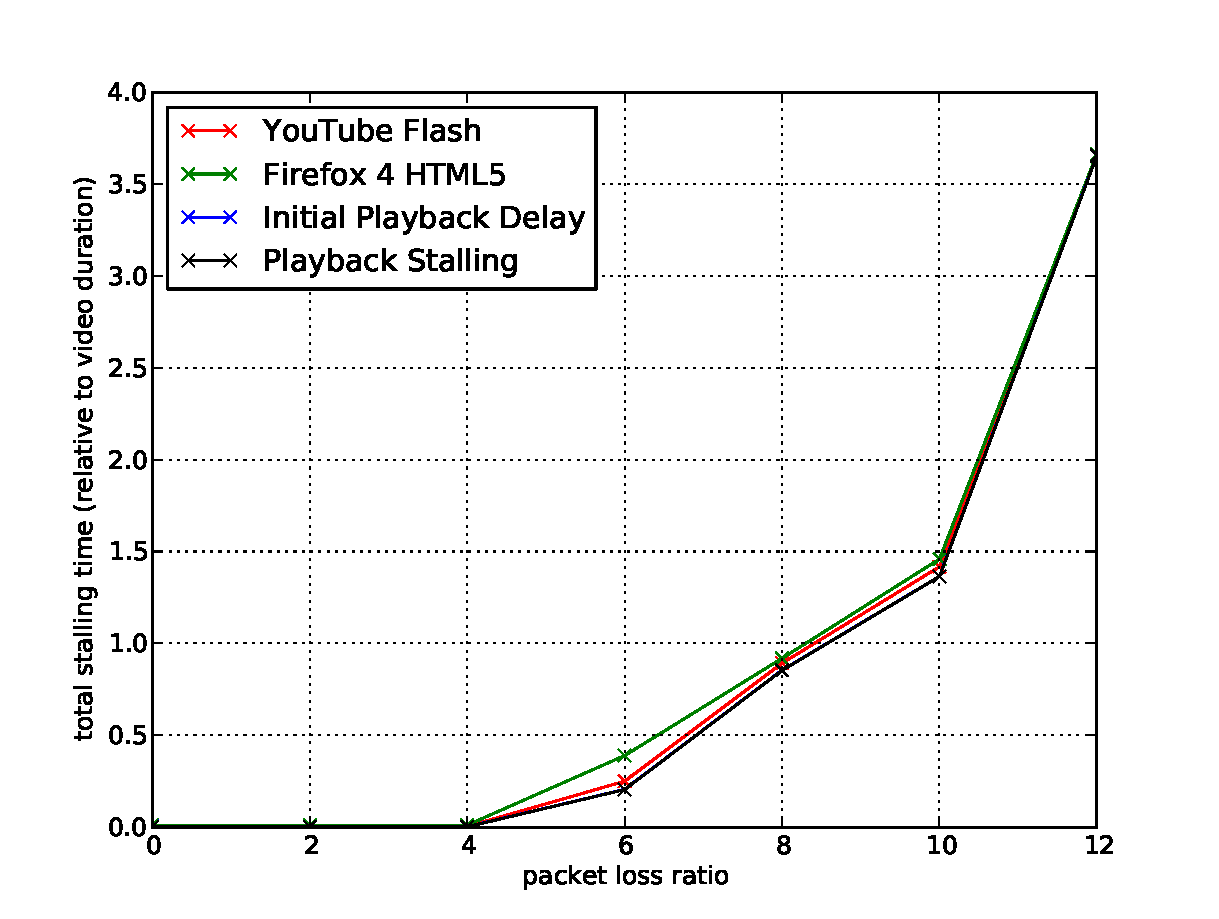
\includegraphics[width=\textwidth]{images/eval-loss4mb-stallingtime.pdf}
    \caption{Playback model observations on additional packet loss. Total stalling time.}
    \label{c3:fig:eval-loss-stallingtime}
\end{figure}

\begin{figure}[htb]
    \centering
    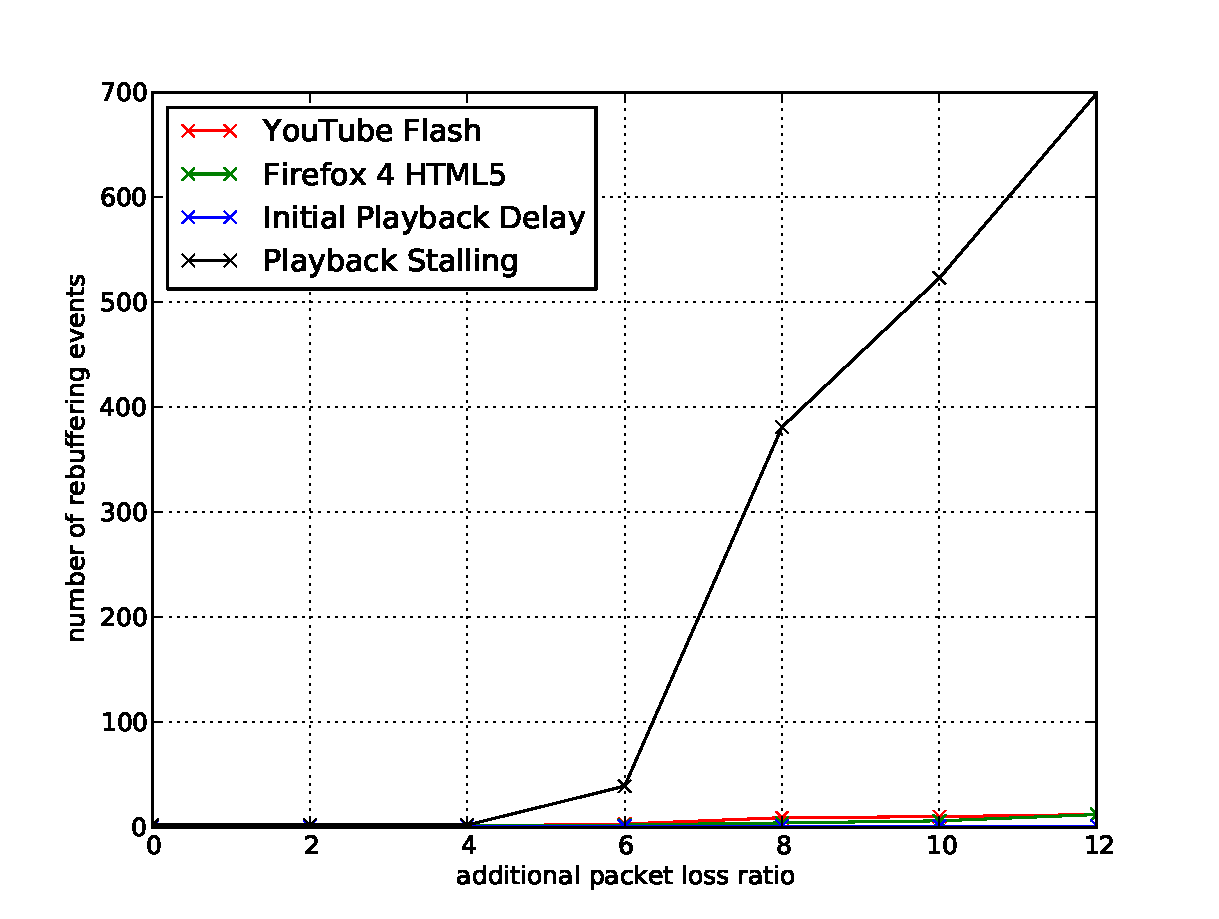
\includegraphics[width=\textwidth]{images/eval-loss4mb-frequency.pdf}
    \caption{Playback model observations on additional packet loss. Number of stalls.}
    \label{c3:fig:eval-loss-numstalls}
\end{figure}
 
Through these to exemplary experiments, we tried to show that network QoS parameters have a direct measurable impact on the application layer, namely on HTTP streaming quality. While the models scale rather well with latency, any HTTP streaming is almost impossible with high packet loss values.
Comparing the presented playback models, we conclude that every model represents a trade-off between several parameters, e.g. as measured here, the number and length of stalls. With the knowledge gained from the experiments, playback models could be tailor-made to best suit certain conditions and user requirements. 

